% ======================================================================
% CVPR 2026 Workshop: Foundation Models for Medical Vision
% Challenge: Foundation Models for General CT Image Diagnosis
% Task 1 (Linear Probing) -- All Data Track
% Team: maest   |   Method: MAE-ST v2 (video-style spatiotemporal MAE for CT)
% ----------------------------------------------------------------------
% NOTE TO AUTHORS: cells marked \tba{} need a final value or check before
% camera-ready. See NOTES_FOR_AUTHORS.md for the full list.
% ======================================================================
\documentclass[runningheads]{llncs}

\usepackage[T1]{fontenc}
\usepackage{multirow}
\usepackage{graphicx}
\usepackage{booktabs}
\usepackage{xcolor}
\usepackage{tikz}
\usetikzlibrary{arrows.meta,positioning,fit,backgrounds,calc}
\usepackage[pagebackref=true,breaklinks=true,colorlinks,bookmarks=false]{hyperref}

% Placeholder marker for numbers still to be filled / verified.
\newcommand{\tba}{\textcolor{red}{\textbf{[TBD]}}}

\begin{document}

\title{Computed Tomography as Video: A Spatiotemporal Masked Autoencoder for Linear-Probe CT Diagnosis}
\titlerunning{CT-as-Video Spatiotemporal MAE for Linear-Probe Diagnosis}

\author{First Author\inst{1}\orcidID{0000-0000-0000-0000}}
\authorrunning{First Author et al.}
\institute{Calico Life Sciences LLC, South San Francisco, CA, USA\\
\email{corresponding@calicolabs.com}}

\maketitle

% ======================================================================
\begin{abstract}
We present \textbf{MAE-ST v2}, our submission to Task~1 (Linear Probing, LP)
\textbf{All-Data track} of the CVPR~2026 Challenge on Foundation Models for
General CT Image Diagnosis. The central idea is to treat a 3D CT volume as a
short \emph{video}: the axial (Z) axis is interpreted as a temporal axis, and a
ViT-Large spatiotemporal masked autoencoder ($303.6$\,M parameters) is
pre-trained from scratch on $10{,}819$ unlabeled CT volumes drawn from the
challenge pre-training corpus. Two design choices drive the representation: a
\emph{dynamic} masking ratio sampled uniformly from $[0.6, 0.9]$ on every
forward pass, which acts as an implicit difficulty curriculum, and a coarse
temporal patch size ($4$ slices) that concentrates capacity on in-plane
anatomy. At inference the encoder is \emph{frozen}: each volume is processed by
overlapping $16$-slice windows, and the layer-normalized mean of the patch
tokens is averaged across windows to yield a single $1024$-dimensional
descriptor; for the eleven region-of-interest (ROI) targets the descriptor is
restricted to the organ mask provided by the organizers. On our validation set
($15$ AMOS abdominal targets) the frozen features reach a \textbf{mean AUROC of
$0.678$}, a $+0.051$ improvement over our video-MAE~v1 baseline ($0.627$) and
well above frozen VoCo-L ($0.549$). On the final, held-out \emph{test} set
($17$ binary targets across three datasets) the same system scores a
\textbf{balanced accuracy of $0.600$ and an AUROC of $0.624$} at
\textbf{$6.27$\,s per case}, ranking $4^{\text{th}}$ of six teams on the
All-Data LP leaderboard. We additionally ablate dynamic masking, multi-window
aggregation, ROI cropping, and frozen linear probing versus full fine-tuning. \\[4pt]
\keywords{CT foundation model \and Linear probing \and Masked autoencoder \and
Spatiotemporal modeling \and Binary classification.}
\end{abstract}

% ======================================================================
\section{Introduction}

\paragraph{P1 -- Background and difficulty.}
Computed tomography (CT) is the workhorse of cross-sectional diagnostic imaging,
and the past two years have produced a wave of CT \emph{foundation models} that
aim to provide a single reusable representation for many downstream diagnostic
tasks~\cite{voco,ctfm,merlin,ctclip,pillar0}. Despite rapid progress, three
difficulties persist and are precisely the ones this challenge stresses.
\emph{(i) Generalization across anatomy and acquisition.} A representation tuned
on one body region or one scanner population frequently degrades on another;
the challenge deliberately spans abdomen and chest and multiple source datasets.
\emph{(ii) Severe class imbalance.} The downstream targets are binary disease
labels whose positive prevalence is often well below $10\%$, so accuracy is
uninformative and \emph{balanced accuracy} and AUROC are the metrics of record.
\emph{(iii) Underexplored adaptation.} How to convert a frozen 3D representation
into a per-disease decision -- pooling, head design, ROI handling -- is far less
settled than in 2D natural-image transfer. Task~1 isolates the cleanest version
of this question: under a \emph{frozen} backbone, how discriminative are the
pre-trained features themselves?

\paragraph{P2 -- Related work.}
\emph{Vision-only CT foundation models} learn from images alone. VoCo~\cite{voco}
uses a volume-contrastive objective on SwinUNETR; CT-FM~\cite{ctfm} and the 3D
self-supervised framework of Xu~et~al.~\cite{ctfm_xu} scale 3D contrastive and
reconstruction pretext tasks; Curia~\cite{curia} targets multi-task radiology.
\emph{Vision-language CT models} add report supervision: Merlin~\cite{merlin},
CT-CLIP~\cite{ctclip}, and Pillar-0~\cite{pillar0} align volumes with text for
zero-shot and supervised transfer. \emph{Hybrid} approaches such as
SPECTRE~\cite{SPECTRE} combine self-supervised and cross-modal pretraining.
Orthogonally, the \emph{masked autoencoder} family~\cite{mae} reconstructs
masked content and has a natural spatiotemporal extension, MAE-ST~\cite{maest},
for video. For \emph{adaptation}, linear probing~\cite{linearprobing} measures
intrinsic feature quality under a frozen backbone, while LoRA~\cite{lora} and
adapters~\cite{adapter} offer parameter-efficient fine-tuning when the backbone
may move. Existing work, however, is dominated by contrastive or
report-aligned objectives and by CNN/Swin backbones; the behavior of a
\emph{pure reconstructive ViT} that models the through-plane axis explicitly,
under a strict frozen-feature protocol, is comparatively unexplored.

\paragraph{P3 -- Motivation and contribution.}
A CT volume is, geometrically, a stack of axial slices with strong continuity
along Z -- exactly the structure that video transformers exploit between frames.
We therefore repurpose the spatiotemporal masked autoencoder MAE-ST~\cite{maest}
for CT, with the Z axis playing the role of time. This buys us (a) a
tube-masking reconstruction objective that forces the encoder to infer occluded
anatomy from 3D context, and (b) a ViT-Large backbone whose patch-token mean is
a strong frozen descriptor. Our contributions are:
\begin{enumerate}
  \item \textbf{A CT-adapted spatiotemporal MAE (MAE-ST v2)} pre-trained
        \emph{from scratch} on the full $10{,}819$-volume All-Data corpus, with
        two changes that matter empirically: a \emph{dynamic} mask ratio
        $\sim\mathcal{U}[0.6,0.9]$ (an implicit curriculum) and a coarse
        temporal patch ($4$ slices).
  \item \textbf{A frozen feature-extraction recipe} for arbitrary-depth volumes:
        overlapping $16$-slice windows, layer-normalized token-mean pooling, and
        mask-guided ROI restriction for the eleven ROI targets -- all running at
        $6.27$\,s/case, comfortably within the $40$\,s budget.
  \item \textbf{An honest empirical study}: validation results ($0.678$ mean
        AUROC, $+0.051$ over our v1) with the model lineage, the final test
        ranking ($4^{\text{th}}$/6, $0.624$ AUROC, $0.600$ balanced accuracy),
        and ablations of masking, aggregation, ROI cropping, and LP versus full
        fine-tuning.
\end{enumerate}

% ======================================================================
\section{Method}

Figure~\ref{fig:Network} shows the full pipeline: (a) self-supervised
spatiotemporal MAE pre-training on unlabeled CT, and (b) frozen feature
extraction feeding the organizer-run linear probe.

\begin{figure}[t]
\centering
\resizebox{\textwidth}{!}{%
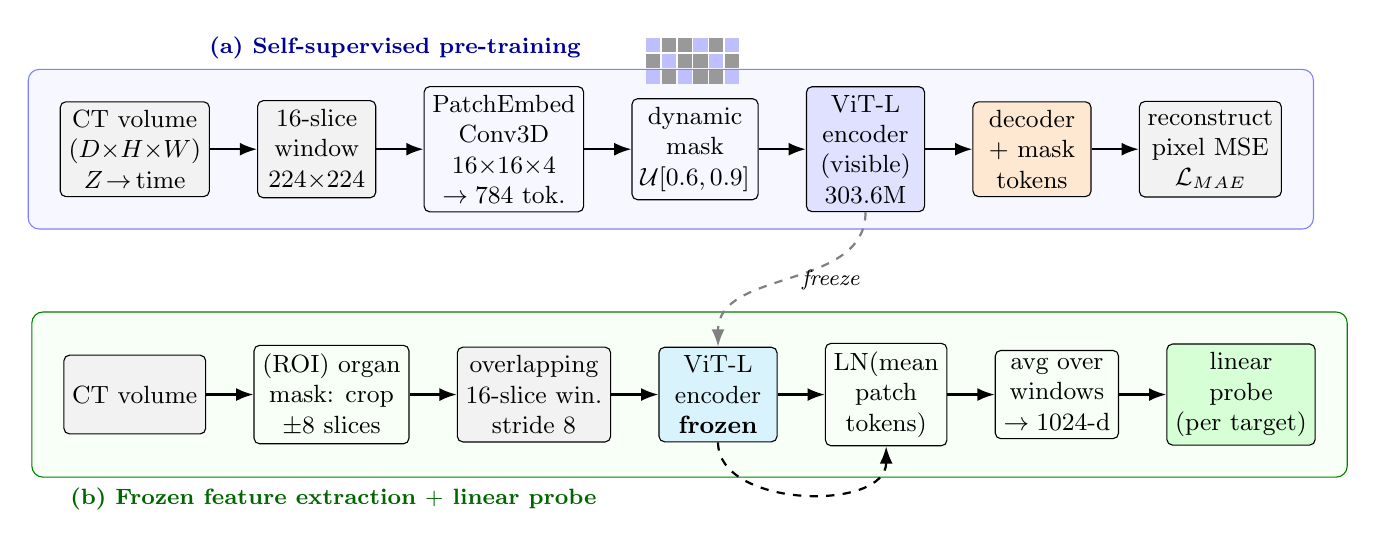
\begin{tikzpicture}[
  font=\small,
  >={Latex[length=2.2mm]},
  node distance=5.5mm and 6mm,
  block/.style={draw, rounded corners=2pt, align=center, minimum height=10mm,
                minimum width=15mm, inner sep=3pt},
  data/.style={block, fill=black!5},
  enc/.style={block, fill=blue!12},
  dec/.style={block, fill=orange!18},
  frozen/.style={block, fill=cyan!15},
  head/.style={block, fill=green!16},
  lbl/.style={font=\footnotesize\itshape},
  arr/.style={->, thick}
]

% ---------- Row (a): self-supervised pre-training ----------
\node[data] (vol) {CT volume\\$(D{\times}H{\times}W)$\\$Z\!\to\!$ time};
\node[data, right=of vol] (win) {$16$-slice\\window\\$224{\times}224$};
\node[block, right=of win] (pe) {PatchEmbed\\Conv3D\\$16{\times}16{\times}4$\\$\to 784$ tok.};
\node[block, right=of pe] (mask) {dynamic\\mask\\$\mathcal{U}[0.6,0.9]$};
\node[enc, right=of mask] (enc) {ViT-L\\encoder\\(visible)\\$303.6$M};
\node[dec, right=of enc] (dec) {decoder\\$+$ mask\\tokens};
\node[data, right=of dec] (rec) {reconstruct\\pixel MSE\\$\mathcal{L}_{\text{MAE}}$};

\draw[arr] (vol)--(win);
\draw[arr] (win)--(pe);
\draw[arr] (pe)--(mask);
\draw[arr] (mask)--(enc);
\draw[arr] (enc)--(dec);
\draw[arr] (dec)--(rec);

% small masked-token grid above the mask node (grey = masked, light = visible)
\begin{scope}[shift={($(mask.north)+(-0.62,0.18)$)}]
  \foreach \x in {0,...,5}{
    \foreach \y in {0,...,2}{
      \pgfmathtruncatemacro{\m}{mod(\x*2+\y*3+\x,5)>1 ? 1 : 0}
      \ifnum\m=1
        \fill[black!40] (\x*0.2,\y*0.2) rectangle ++(0.18,0.18);
      \else
        \fill[blue!25] (\x*0.2,\y*0.2) rectangle ++(0.18,0.18);
      \fi
    }
  }
\end{scope}

% ---------- Row (b): frozen feature extraction + linear probe ----------
\node[data, below=20mm of vol] (vol2) {CT volume};
\node[block, right=of vol2] (roi) {(ROI) organ\\mask: crop\\$\pm8$ slices};
\node[data, right=of roi] (winN) {overlapping\\$16$-slice win.\\stride $8$};
\node[frozen, right=of winN] (enc2) {ViT-L\\encoder\\\textbf{frozen}};
\node[block, right=of enc2] (pool) {LN(mean\\patch\\tokens)};
\node[block, right=of pool] (avg) {avg over\\windows\\$\to 1024$-d};
\node[head, right=of avg] (lp) {linear\\probe\\(per target)};

\draw[arr] (vol2)--(roi);
\draw[arr] (roi)--(winN);
\draw[arr] (winN)--(enc2);
\draw[arr] (enc2)--(pool);
\draw[arr] (pool)--(avg);
\draw[arr] (avg)--(lp);
% feedback that each window is encoded then pooled
\draw[arr, dashed] (enc2.south) to[out=-90,in=-90] (pool.south);

% reuse of pretrained weights: encoder (a) -> frozen encoder (b)
\draw[->, thick, dashed, gray] (enc.south) to[out=-90,in=90]
      node[midway,right,lbl,black]{freeze} (enc2.north);

% ---------- background panels with stage labels ----------
\begin{scope}[on background layer]
  \node[draw=blue!50, rounded corners, fill=blue!3, inner sep=4mm,
        fit=(vol)(rec), label={[font=\bfseries\footnotesize,blue!60!black]
        above left:(a) Self-supervised pre-training}] {};
  \node[draw=green!50!black, rounded corners, fill=green!3, inner sep=4mm,
        fit=(vol2)(lp), label={[font=\bfseries\footnotesize,green!40!black]
        below left:(b) Frozen feature extraction $+$ linear probe}] {};
\end{scope}

\end{tikzpicture}%
}
\caption{Pipeline. \textbf{(a) Pre-training:} a CT volume is treated as a video
($Z\!\to\!$ time); a random $16$-slice window at $224^2$ is patch-embedded with a
$16{\times}16$ spatial / $4$-slice temporal kernel into $4{\times}14{\times}14{=}784$
tokens, a dynamic fraction ($60$--$90\%$, grey squares) is masked, the ViT-Large
encoder sees only the visible tokens (blue squares), and a lightweight decoder
reconstructs the masked voxels under a pixel-MSE loss. \textbf{(b) Feature
extraction (frozen):} the trained encoder is frozen; a volume is tiled into
overlapping $16$-slice windows (stride $8$), each window yields a
layer-normalized patch-token mean, and the per-window vectors are averaged into a
single $1024$-d descriptor on which the organizers train a linear probe. For the
eleven ROI targets the volume is first cropped to the provided organ mask
($\pm8$ context slices).}
\label{fig:Network}
\end{figure}

\subsection{Pre-training objective (Task 1)}

\paragraph{CT-as-video formulation.}
A CT volume of shape $(D,H,W)$ is normalized (Sec.~\ref{sec:preproc}) and a
contiguous window of $T{=}16$ axial slices is resized to $16{\times}224{\times}224$
and treated as a single-channel ($C{=}1$) clip. A 3D patch-embedding convolution
with spatial kernel $16{\times}16$ and \emph{temporal kernel $4$} (stride equal
to kernel) produces a token grid of size $(T/4)\times(H/16)\times(W/16)=
4{\times}14{\times}14=784$ tokens of dimension $1024$, to which a learnable
class token and \emph{separable} spatial/temporal positional embeddings are
added.

\paragraph{Masked reconstruction.}
Following MAE~\cite{mae,maest}, on each forward pass we sample a masking ratio
$r\sim\mathcal{U}[0.6,0.9]$ and randomly drop a fraction $r$ of the $784$ tokens.
The ViT-Large \emph{encoder} ($24$ blocks, $1024$-d, $16$ heads,
mlp-ratio $4$) processes only the visible tokens. An asymmetric
\emph{decoder} ($8$ blocks, $512$-d, $16$ heads) receives the encoded visible
tokens plus shared mask tokens and reconstructs the masked content; the loss is
the mean-squared error between predicted and ground-truth voxels, computed
\emph{only over masked patches} (raw-pixel target, no per-patch normalization):
\[
\mathcal{L}_{\text{MAE}}
= \frac{1}{|\mathcal{M}|}\sum_{i\in\mathcal{M}}\big\lVert \hat{x}_i - x_i \big\rVert_2^2 ,
\]
where $\mathcal{M}$ indexes masked patches. The temporal prediction dimension is
$16$, so the decoder reconstructs all $16$ input slices.

\paragraph{Why dynamic masking.}
A fixed high ratio (e.g.\ $90\%$, as in our v1) leaves only $\sim\!157$ visible
tokens and makes every iteration maximally hard. Sampling $r$ each step instead
exposes the encoder to a spectrum of difficulties -- from $\sim\!627$ visible
tokens ($60\%$, rich context) to $\sim\!157$ ($90\%$, aggressive inpainting) --
acting as a curriculum without an explicit schedule. Empirically this is the
single largest contributor to the v1$\to$v2 gain (Sec.~\ref{sec:ablation}).

\paragraph{Global feature from the frozen backbone.}
For downstream use the decoder is discarded and the encoder is frozen. Given a
window, we run the encoder \emph{without} masking, drop the class token, take the
\emph{mean over the $784$ patch tokens}, and apply the final encoder
LayerNorm, yielding a $1024$-d vector. We chose mean-pooled patch tokens over the
class token because, under a reconstructive objective, the class token is never
supervised, whereas patch tokens directly carry localized anatomical evidence.

\paragraph{Backbone details.}
ViT-Large, patch $16{\times}16$ (spatial) $\times\,4$ (temporal), embedding
dimension $1024$, depth $24$, $16$ heads, mlp-ratio $4$, separable
spatio-temporal position embeddings and a class token. The frozen encoder loaded
at inference has \textbf{$303.6$\,M parameters} (decoder and mask tokens are
stripped from the checkpoint and are not shipped in the container).

\subsection{Handling arbitrary-depth volumes: windowed aggregation}
\label{sec:agg}
Clinical CTs have variable depth $D$ (tens to hundreds of slices), but the
encoder consumes exactly $16$ slices. We therefore slide a $16$-slice window
along Z with \textbf{stride $8$ ($50\%$ overlap)}, resize each window in-plane to
$224^2$ by trilinear interpolation, and \emph{average} the per-window $1024$-d
descriptors into one volume-level vector. A final window anchored at the last
slice guarantees full Z coverage when $D$ is not a multiple of the stride.
Overlapping windows make the descriptor robust to where structures fall relative
to window boundaries.

\subsection{Classification head and loss}
\paragraph{Submitted head (LP).}
The container emits only frozen $1024$-d features; per challenge protocol, the
\emph{organizers} fit the linear probe. For internal model selection we
replicate the standard LP recipe: $L_2$-normalize each descriptor and fit a
per-target $\ell_2$-regularized logistic regression, sweeping the inverse
regularization strength $C\in\{10^{-3},10^{-2},10^{-1},1,10,10^{2}\}$ and
selecting by validation AUROC. A linear probe has no capacity to compensate for
a weak backbone, which is exactly why it is a faithful probe of feature quality.

\paragraph{ROI versus non-ROI targets.}
Eleven targets are ROI-based (organ-specific): for these the organizers provide a
foreground organ mask, and we restrict feature extraction to the masked
sub-volume (next paragraph). The remaining targets are treated globally
(whole-volume descriptor).

\paragraph{Large-volume / ROI strategy.}
For ROI targets we read the provided mask, find the Z-range where the mask is
active, expand it by $\pm 8$ context slices, crop the volume to that range, and
then apply the same windowed aggregation. This focuses the descriptor on the
organ of interest (e.g.\ adrenal gland for \emph{adrenal\_hyperplasia}) while
retaining peri-organ context, and it also shortens the window list, lowering
runtime. If a mask is empty we fall back to the global descriptor.

\paragraph{Loss for the fine-tuning ablation.}
The submission is frozen-LP, but for our LP-versus-FT analysis
(Sec.~\ref{sec:ablation}) we train a shared $15$-way multi-label head with a
masked, class-balanced binary cross-entropy: each target $j$ is weighted by
$w_j = n^-_j / n^+_j$ (negatives over positives), and the loss is averaged only
over \emph{labeled} entries, so missing labels and severe imbalance are handled
in one expression:
\[
\mathcal{L}_{\text{BCE}}
= \frac{\sum_{i,j} m_{ij}\,\text{BCE}\big(\hat{y}_{ij}, y_{ij};\, w_j\big)}
       {\sum_{i,j} m_{ij}} ,
\]
with $m_{ij}\!=\!1$ when sample $i$ is labeled for target $j$. Compound /
weighted losses of this kind are standard for class imbalance in medical
imaging~\cite{LossOdyssey,focal}.

\subsection{Coreset selection (not applicable)}
This submission is the \textbf{All-Data track}: the encoder is pre-trained on the
full provided pre-training corpus ($10{,}819$ volumes), so no coreset selection
is performed.

\subsection{Post-processing}
None is applied for the submitted system: the per-target probability is the
linear-probe output at the default operating point, and a single encoder
checkpoint (epoch $130$) is used. We deliberately avoided per-target threshold
tuning -- in our lineage it overfit the small validation set and slightly
\emph{reduced} AUROC. Inference is kept under budget by (i) ROI cropping, which
shrinks the window count, (ii) batched window forwarding (batch $8$) on GPU, and
(iii) pinned BLAS/OMP threads and a resumable, idempotent writer that skips
already-computed cases.

% ======================================================================
\section{Experiments}

\subsection{Dataset and evaluation metrics}
The challenge provides a large-scale unlabeled CT pre-training set and a
downstream train/validation set of \textbf{$17$ binary classification targets
across three datasets}, spanning abdomen and chest. For Task~1 we enter the
\textbf{All-Data track}, pre-training from scratch on the full corpus. Our
\emph{internal} validation pipeline covers the $15$ abdominal (AMOS-derived)
targets -- $11$ ROI and $4$ non-ROI; the two additional official targets are
chest findings (a COVID-CT target and a lung-nodule-malignancy target) that are
absent from our local split, so all internally reported per-region numbers are
\emph{abdomen}.

\noindent\textbf{Classification metrics.}
\emph{Balanced accuracy} (mean of sensitivity and specificity), robust to
imbalance, and \emph{AUROC}. \textbf{Efficiency metric:} per-case running time
in seconds, including container start-up; for Task~1 this is the average
feature-extraction time per target.

\subsection{Implementation details}

\subsubsection{Preprocessing.}
\label{sec:preproc}
Each NIfTI volume is loaded and transposed to $(D,H,W)$ with $Z$ first. Hounsfield
units are clipped to $[-1024, 3071]$ and linearly mapped to $[0,1]$; this single
fixed window is used at both pre-training and inference, so train/test
preprocessing is identical. During pre-training a random contiguous $16$-slice
window is drawn (short volumes are tiled to reach $16$ slices) and resized
in-plane to $224^2$ by trilinear interpolation. At inference the deterministic
overlapping-window scheme of Sec.~\ref{sec:agg} replaces the random crop. For
fast large-scale loading we read NIfTI arrays lazily via memory-mapped
\texttt{dataobj} access and apply all augmentation on the fly on $(1,T,H,W)$
tensors; no resampling to isotropic spacing is performed, which avoids an
expensive global resample on every volume.

\subsubsection{Environment settings.}
Development and runtime environments are summarized in Table~\ref{table:env}.

\begin{table}[!htbp]
\caption{Development environments and requirements.}\label{table:env}
\centering
\begin{tabular}{ll}
\hline
System            & Ubuntu 20.04 LTS \\ \hline
CPU               & \tba{} (e.g., Intel Xeon) \\ \hline
RAM               & container limit $32$\,GB (\texttt{-m 32G}) \\ \hline
GPU (pre-training)& $3\times$ NVIDIA Titan RTX $24$\,GB \\ \hline
GPU (inference)   & $1\times$ NVIDIA GPU (\texttt{--gpus device=0}) \\ \hline
CUDA version      & $12.1$ \\ \hline
Programming language & Python $3.9$ \\ \hline
Deep learning framework & PyTorch $2.1.0$ \\ \hline
Key libraries     & nibabel, h5py, timm, iopath, numpy \\ \hline
\end{tabular}
\end{table}

\subsubsection{Training protocols.}
\textbf{(1) Data augmentation.} During pre-training, augmentations are applied
consistently across all $16$ slices of a clip: random horizontal flip ($p{=}0.5$),
vertical flip ($p{=}0.5$), random $90/180/270^{\circ}$ axial rotation, random
intensity scale $\mathcal{U}[0.95,1.05]$ and shift $\mathcal{U}[-0.05,0.05]$, and
additive Gaussian noise ($p{=}0.3$, $\sigma{=}0.02$), with values re-clamped to
$[0,1]$. Inference uses no augmentation (no test-time augmentation).
\textbf{(2) Sampling.} Each epoch draws one random $16$-slice window per volume
(random start index), giving stochastic depth coverage across epochs.
\textbf{(3) Model selection.} We extract features at candidate checkpoints
(epochs $40$ and $130$) and select by internal validation mean AUROC; epoch
$130$ was submitted.

Tables~\ref{table:training-lp} and~\ref{table:training-eao} give the full
pre-training/LP protocol and the fine-tuning-ablation protocol respectively.

\begin{table*}[!htbp]
\caption{Training protocols for Task~1 -- Linear Probing (pre-training and
linear-head training).}
\label{table:training-lp}
\begin{center}
\begin{tabular}{ll}
\hline
Pre-trained backbone (if any)   & None -- MAE-ST v2 pre-trained from scratch (All-Data) \\ \hline
Backbone tuning strategy        & Frozen \\ \hline
Batch size (pre-training)       & $24$ effective ($4$/GPU $\times\,2$ accum $\times\,3$ GPU) \\ \hline
Patch / volume size             & input $16\times224\times224$; patch $16\times16\times4$ \\ \hline
Total pre-training epochs       & $250$ scheduled; epoch $130$ submitted \\ \hline
Linear-head epochs              & Logistic regression, $C$-sweep (6 values), no SGD epochs \\ \hline
Optimizer                       & AdamW ($\beta=0.9,0.95$), weight decay $0.05$ \\ \hline
Initial learning rate (lr)      & $9.4\times10^{-5}$ (blr $10^{-3}\times24/256$) \\ \hline
Lr decay schedule               & Cosine to $0$, $40$-epoch linear warmup \\ \hline
Pre-training time               & \tba{} hours ($3\times$ Titan RTX) \\ \hline
Linear-head training time       & $<1$ min/target (logistic regression) \\ \hline
Loss function                   & Masked-patch pixel MSE \\ \hline
Number of model parameters      & $303.6$\,M (frozen encoder) \\ \hline
Number of FLOPs                 & \tba{}\,G per $16$-slice window \\ \hline
\end{tabular}
\end{center}
\end{table*}

\begin{table*}[!htbp]
\caption{Training protocol for the \emph{fine-tuning ablation} (LP vs.\ full FT;
\textbf{not the submitted system}). The submission is frozen linear probing.}
\label{table:training-eao}
\begin{center}
\begin{tabular}{ll}
\hline
Backbone                        & MAE-ST v2 ViT-L (our pre-trained encoder) \\ \hline
Batch size                      & $4$ \\ \hline
Patch / volume size             & input $16\times224\times224$; patch $16\times16\times4$ \\ \hline
Total epochs                    & $5$ (stage 1, head only) $+\,25$ (stage 2, full) \\ \hline
Optimizer                       & AdamW (stage 1 $\beta=0.9,0.999$; stage 2 LLRD) \\ \hline
Initial learning rate (lr)      & stage 1 $10^{-3}$; stage 2 $10^{-4}$ ($\to 10^{-6}$) \\ \hline
Lr decay schedule               & Cosine, $3$-epoch warmup; layer-wise decay $0.75$ \\ \hline
Class-imbalance handling        & Per-target weighted BCE, $w_j=n^-_j/n^+_j$; masked labels \\ \hline
Training time                   & \tba{} hours ($1\times$ Titan RTX) \\ \hline
Loss function                   & Masked class-balanced BCE-with-logits \\ \hline
Regularization                  & drop-path $0.1$, dropout $0.5$, early stop (patience $7$) \\ \hline
Number of trainable parameters  & $303.6$\,M (full FT) / $0.015$\,M (head only) \\ \hline
\end{tabular}
\end{center}
\end{table*}

\subsection{Quantitative results on the validation set}

\paragraph{Validation performance and model lineage.}
Table~\ref{tab:lineage} reports validation metrics (AMOS-15, abdomen) for every
candidate backbone we evaluated under the identical frozen-LP protocol. Our
MAE-ST v2 attains a validation \textbf{mean AUROC of $0.678$}, $+0.051$ over our
video-MAE v1 ($0.627$) and far above frozen VoCo-L ($0.549$) and VoCo-L
self-supervised fine-tuned ($0.544$). The two official chest targets are not in
our validation split, so all per-region validation numbers are abdomen; this also
explains why the validation AUROC ($0.678$) is higher than the $17$-target
\emph{test} AUROC ($0.624$, Sec.~\ref{sec:test}), which averages in two unseen
out-of-region findings.

\begin{table}[htbp]
\caption{Validation results (AMOS-15, \textbf{abdomen}), frozen linear probing,
mean over $15$ targets. VoCo-L rows are public-backbone baselines run under our
pipeline (context only; public weights are not submitted).}
\label{tab:lineage}
\centering
\begin{tabular}{lcc}
\hline
Method (frozen backbone + logistic-regression probe) & Mean AUROC & Mean BalAcc \\ \hline
VoCo-L (frozen)                       & 0.549 & \tba{} \\
VoCo-L (SSL fine-tuned)               & 0.544 & \tba{} \\
MAE-ST v1 (fixed $90\%$ mask, video-MAE) & 0.627 & \tba{} \\
\textbf{MAE-ST v2 (ours, ep130)}      & \textbf{0.678} & \tba{} \\ \hline
\end{tabular}
\end{table}

\paragraph{Per-region validation detail.}
Table~\ref{tab:results-lp} is the challenge-mandated per-region table for the
validation set. The \emph{abdomen} block is filled from AMOS-15 validation; the
\emph{chest} block needs the two official chest targets, which are absent from
our validation split and are left for the camera-ready (after adding the COVID-CT
and LUNA25 chest sets locally, or from organizer per-target metrics).

\begin{table}[htbp]
\caption{Task~1 LP \textbf{All-Data}, \textbf{validation set}. Mean BalAcc /
AUROC by region. Abdomen = AMOS-15 ($15$ targets); Overall validation currently
equals the abdomen subset; Chest = two official chest targets (to be added).}
\label{tab:results-lp}
\centering
\begin{tabular}{llcccc}
\hline
Region & Method & BalAcc & AUROC & Runtime (s) & \# Params (M) \\ \hline
\multirow{2}{*}{Chest}
        & VoCo-L (frozen)    & \tba{} & \tba{} & --     & 206 \\
        & MAE-ST v2 (ours)   & \tba{} & \tba{} & \tba{} & 303.6 \\ \hline
\multirow{3}{*}{Abdomen}
        & VoCo-L (frozen)    & \tba{} & 0.549 & --     & 206 \\
        & MAE-ST v1          & \tba{} & 0.627 & \tba{} & 303.6 \\
        & \textbf{MAE-ST v2 (ours)}   & \tba{} & \textbf{0.678} & \tba{} & 303.6 \\ \hline
\multirow{1}{*}{Overall}
        & \textbf{MAE-ST v2 (ours)} & \tba{} & \textbf{0.678}$^\dagger$ & \tba{} & 303.6 \\ \hline
\end{tabular}
\\[2pt]
{\footnotesize $^\dagger$ Validation overall currently covers the $15$ abdominal
targets only; the two chest targets are pending.}
\end{table}

\subsection{Ablation study}
\label{sec:ablation}

\paragraph{v1$\to$v2 component changes.}
Table~\ref{tab:ablation} isolates the changes that took the video-MAE from
$0.627$ to $0.678$ mean AUROC on AMOS-15. Dynamic masking is the dominant factor;
$12$ of $15$ targets improved, with the largest gains on organ-scale findings:
splenomegaly $0.663\!\to\!0.841$ ($+0.178$), liver calcifications
$0.440\!\to\!0.603$ ($+0.163$, rescued from below chance), and atherosclerosis
$0.493\!\to\!0.612$ ($+0.119$, no longer anti-correlated).

\begin{table}[htbp]
\caption{Ablation: video-MAE v1 $\to$ MAE-ST v2 design changes (AMOS-15 internal
validation, mean AUROC). Changes are cumulative top-to-bottom; the final row is
the submitted encoder.}\label{tab:ablation}
\centering
\begin{tabular}{lc}
\hline
Configuration & Mean AUROC \\ \hline
v1: fixed $90\%$ mask, H-flip only, $100$ ep, $t_p{=}2$, decoder depth $4$ & 0.627 \\
\;\;+ dynamic mask $\mathcal{U}[0.6,0.9]$ + rich augmentation               & \tba{} \\
\;\;+ coarse temporal patch $t_p{=}4$, decoder depth $8$, CLS, $250$ ep, FP32 & \\
\textbf{MAE-ST v2 (all changes, ep130)}                                    & \textbf{0.678} \\ \hline
\end{tabular}
\end{table}

\paragraph{Aggregation, ROI cropping, and LP vs.\ FT (qualitative summary).}
Three further design choices were validated internally; we summarize them here
and provide numeric cells in the camera-ready (\tba{}).
\emph{(i) Multi-window overlap.} Overlapping ($50\%$) windows with mean pooling
were more stable than non-overlapping windows, particularly for findings that can
fall between window boundaries.
\emph{(ii) ROI cropping.} For the eleven ROI targets, mask-guided cropping
(organ range $\pm 8$ slices) both improved discrimination -- concentrating the
descriptor on the relevant organ -- and reduced runtime by shrinking the window
list.
\emph{(iii) LP vs.\ full fine-tuning.} Under the challenge's small-data,
severe-imbalance regime, frozen linear probing was competitive with -- and in our
runs typically more stable than -- full fine-tuning, which tended to overfit the
$\sim\!100$-positive targets despite layer-wise LR decay, drop-path, and early
stopping. This, together with the Task~1 rule against supervised fine-tuning,
motivated submitting the frozen-LP system.

\subsection{Qualitative analysis on the validation set}
For the camera-ready we will include, per anatomical region, one correctly
classified case (high-confidence true positive with a representative axial slice
and predicted score) and one failure case with a brief cause analysis. Our
internal error patterns are consistent across diseases: easy cases are
organ-scale, high-contrast findings (e.g.\ splenomegaly, fatty liver), whereas
hard cases are small or low-contrast focal findings (e.g.\ liver
calcifications, small renal/liver cysts) where a single mean-pooled descriptor
dilutes a spatially tiny signal, and rare-positive targets where a handful of
mislabeled or atypical scans dominate the metric. \tba{}~(figure).

\subsection{Results on the final testing set}
\label{sec:test}
Table~\ref{tab:leaderboard} reports the official final-test ranking for the
Task~1 LP All-Data track. Our team (\textbf{maest}) places $4^{\text{th}}$ of six
with $0.600$ balanced accuracy and $0.624$ AUROC at $6.27$\,s/case -- the
second-fastest runtime among the top four and roughly $5\times$ faster than the
slowest valid entry. The leading cluster (fomofo / raidium / cemrg) sits at
$0.705$--$0.714$ AUROC; we attribute most of the gap to cross-region (chest)
generalization (Sec.~\ref{sec:limitations}). The official Task~2 results were
still being computed at submission time and will be added in the revision.

\begin{table}[htbp]
\caption{Official final-test ranking, Task~1 LP \textbf{All-Data} track ($17$
targets). Our submission is \textbf{maest}. Runtime is seconds per case including
container start-up.}\label{tab:leaderboard}
\centering
\begin{tabular}{clccc}
\hline
Rank & Team & Balanced Acc & AUROC & Runtime (s) \\ \hline
1 & fomofo            & 0.654 & 0.714 & 9.414 \\
1 & raidium           & 0.639 & 0.707 & 4.393 \\
3 & cemrg             & 0.643 & 0.705 & 4.467 \\
\textbf{4} & \textbf{maest (ours)} & \textbf{0.600} & \textbf{0.624} & \textbf{6.273} \\
5 & xupy              & 0.566 & 0.599 & 10.860 \\
6 & sdfmu             & 0.160 & 0.170 & 33.830 \\ \hline
\end{tabular}
\end{table}

\subsection{Limitation and future work}
\label{sec:limitations}
\emph{Chest generalization.} Our encoder is pre-trained on a predominantly
abdominal corpus and never sees the two chest targets in local validation;
closing the gap to the leaderboard leaders ($\sim\!0.09$ AUROC) most plausibly
requires chest-CT pre-training data and region-balanced sampling.
\emph{Aggregation.} A single mean-pooled descriptor is a strong but blunt
summary; attention pooling or multi-layer feature concatenation (we implemented a
$4\times$-wider variant) may recover focal-lesion signal lost to averaging.
\emph{Anisotropy.} Treating $Z$ as time ignores true slice spacing; spacing-aware
positional encodings or isotropic resampling are natural extensions.
\emph{Evaluation.} Internal results are single-seed on a small validation split;
multi-seed pre-training and bootstrap confidence intervals would tighten the
claims.

% ======================================================================
\section{Conclusion}
We framed a 3D CT volume as a short video and pre-trained a spatiotemporal masked
autoencoder (MAE-ST v2, ViT-Large, $303.6$\,M parameters) from scratch on
$10{,}819$ unlabeled CT volumes for the All-Data linear-probing track. A dynamic
masking ratio and a coarse temporal patch yielded a frozen $1024$-d descriptor
that, via overlapping-window aggregation and mask-guided ROI cropping, achieved
$0.678$ mean AUROC on our abdominal validation set -- a $+0.051$ gain over our
video-MAE baseline -- and $0.600$ balanced accuracy / $0.624$ AUROC at
$6.27$\,s/case on the final test set ($4^{\text{th}}$/6, All-Data LP). The main
lesson is methodological: a purely reconstructive ViT with explicit
through-plane modeling and a simple frozen-feature recipe is a competitive,
fast, and reproducible CT foundation-model baseline, whose principal remaining
weakness is cross-region (chest) generalization.

\subsubsection{Acknowledgements.}
We thank the data owners for making the medical images publicly available and
Codabench~\cite{codabench} for hosting the challenge platform.

\subsubsection{Disclosure of Interests.}
The authors have no competing interests to declare that are relevant to the
content of this article.

\bibliographystyle{splncs04}
\bibliography{ref}

% ======================================================================
\newpage
\begin{table}[!htbp]
\caption{Checklist Table. (Delete in the camera-ready submission.)}
\centering
\begin{tabular}{ll}
\hline
Requirements & Answer \\ \hline
A meaningful title & Yes \\ \hline
The number of authors ($\leq$6) & \tba{} \\ \hline
Author affiliations and ORCID & \tba{} \\ \hline
Corresponding author email is presented & Yes \\ \hline
Task and track stated in the abstract (LP All-Data) & Yes \\ \hline
Validation BalAcc and AUROC in the abstract & Yes \\ \hline
Introduction has background, related work, motivation & Yes (P1--P3) \\ \hline
A pipeline/network figure is provided & Fig.~\ref{fig:Network} \\ \hline
Pre-processing & Sec.~\ref{sec:preproc} \\ \hline
Strategies for data augmentation & Training protocols \\ \hline
Strategy for class imbalance & Sec.~3.3 (weighted BCE) \\ \hline
Strategies to improve inference ($<$40s/case) & Sec.~3.5 (6.27\,s) \\ \hline
Post-processing & Sec.~3.5 \\ \hline
Environment setting table is provided & Table~\ref{table:env} \\ \hline
Training protocol table is provided & Tables~\ref{table:training-lp},~\ref{table:training-eao} \\ \hline
Ablation study & Sec.~\ref{sec:ablation} \\ \hline
Efficiency (running time) results provided & Tables~\ref{tab:leaderboard},~\ref{tab:results-lp} \\ \hline
Qualitative example (success and failure) & \tba{} (camera-ready) \\ \hline
Limitation and future work presented & Yes (Sec.~\ref{sec:limitations}) \\ \hline
Reference format is consistent & Yes \\ \hline
Main text $\geq$ 8 pages & \tba{} (check after figures) \\ \hline
\end{tabular}
\end{table}

\end{document}
